% Pour faire une référence d'une annexe
% (Annexe \ref{sec:nomsection} page~\pageref{sec:nomsection})

\section{Histoire de la notation musicale : exemple de texte neumé}
\label{sec:exempleTexteNeume}
\begin{figure}[!htbp]
	\centering
	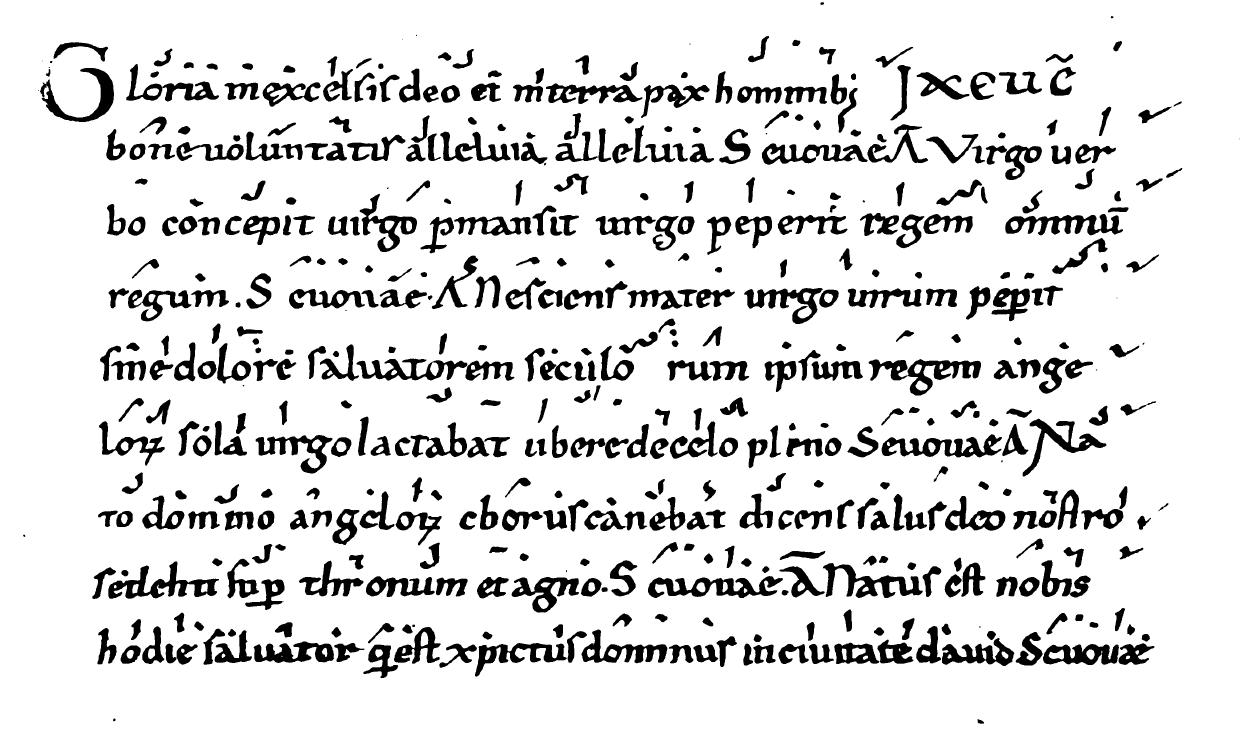
\includegraphics[keepaspectratio=true, width=\textwidth]{Annexes/i/neumes.jpg}
	\caption{Exemple de texte neumé - Source : 1774, Martin Gerbert, \textit{De cantu et musica sacra a prima Ecclesiae aetate usque ad praesens Tempus}, St. Blasien, Typis San-Blasianis, t. I, t. II. - \textit{Les neumes sont les symboles inscrient au-dessus des mots du chant liturgique (ici le chant} Gloria \textit{de l'ordinaire de la messe).} }
	\label{fig:neumes}
\end{figure}
\clearpage

\section{Histoire de la notation musicale : exemple de notation carrée}
\label{sec:exempleNotationCarree}
\begin{figure}[H]
	\centering
	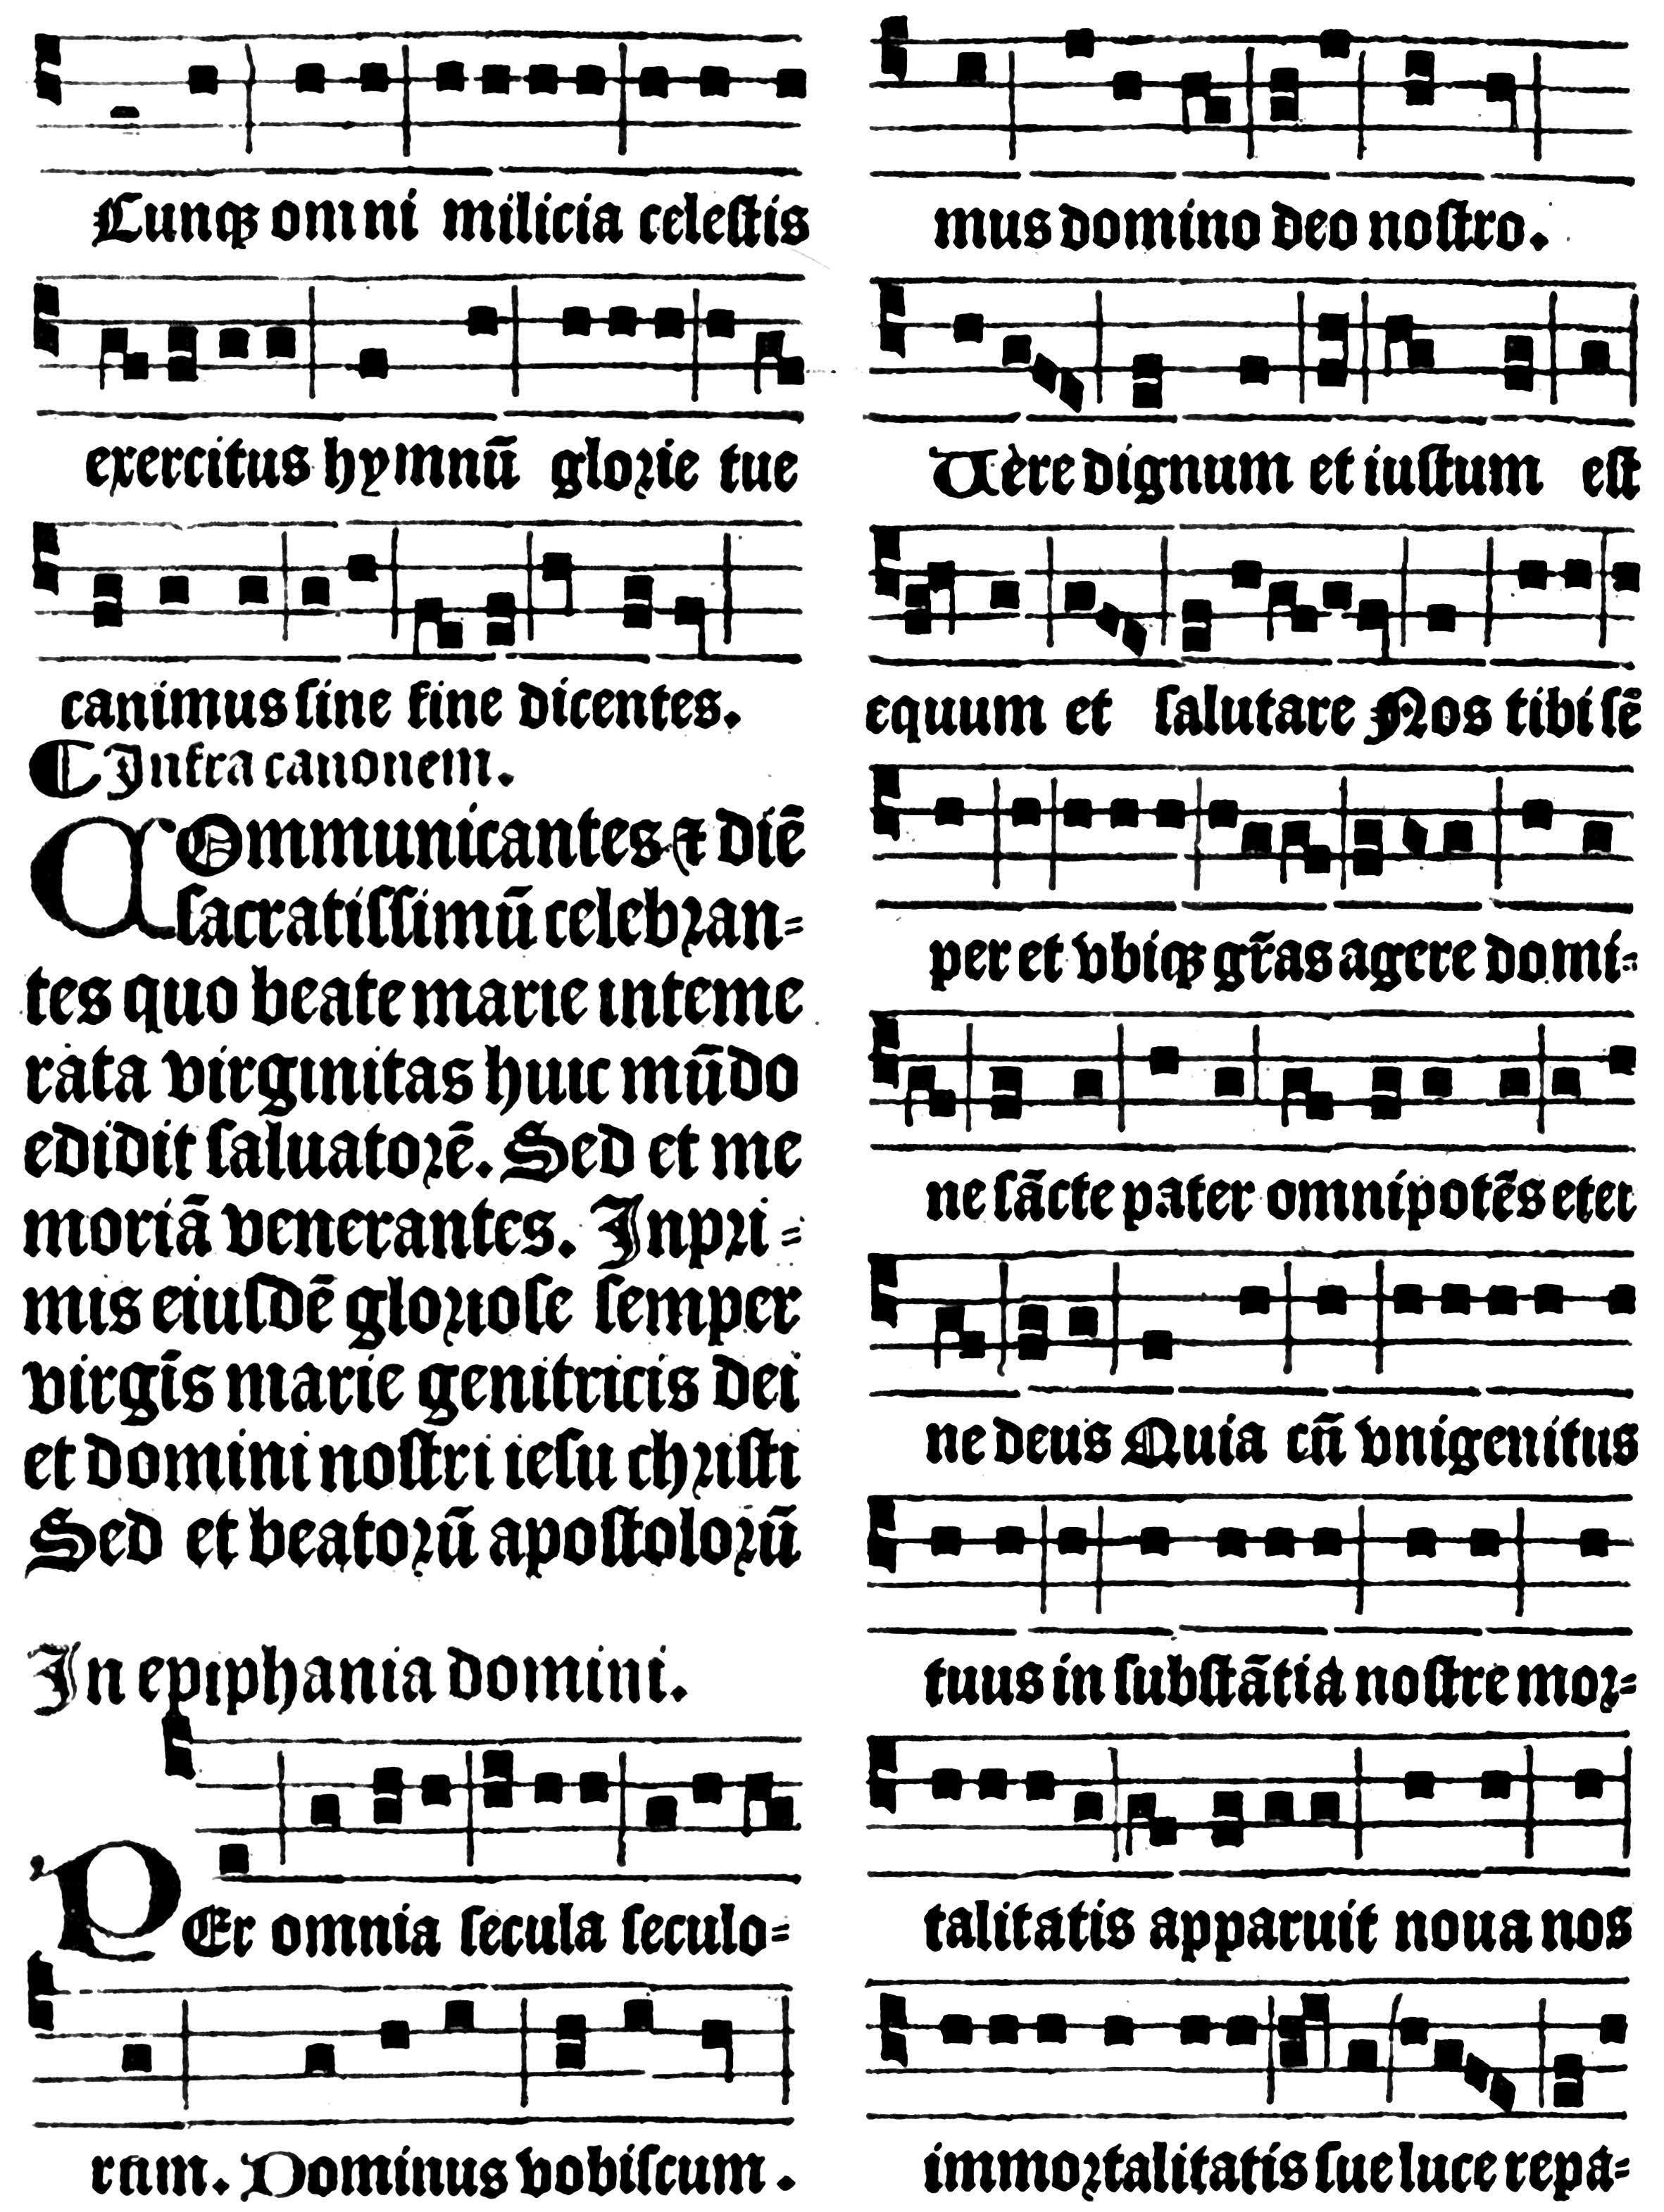
\includegraphics[keepaspectratio=true, width=\textwidth]{Notation/i/notationCarree.jpg}
	\caption{Exemple de notation carrée "imprimée" - Source : 1499, Jean Highman, \textit{Missale Leodiense}, Paris - \textit{Les notes sont représentées en notation carrée toujours au-dessus du texte chanté.} }
	\label{fig:notationCarree}
\end{figure}
